\begin{figure}[t]

\centering

% \subcaptionbox{Comparison in loss surface view\label{fig:diff}}{
%     \includegraphics[width=0.27\textwidth]{figures/swa_vs_swad.pdf}
% (a) The extent of flat region depends on the degree of shaking defined as flat. Thanks to constant learning rate and densely averaging, SWAD catches the center of the wider flat region accurately. Relatively, SWA cannot provide enough robustness to domain shifts because it finds a solution in the narrow flat region.
% }\quad
\begin{subfigure}{0.4\linewidth}
    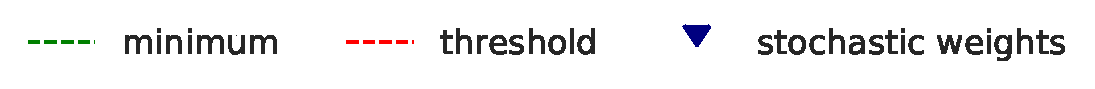
\includegraphics[width=\linewidth]{figures/swad_concept/conceptfig_legend.pdf}
\end{subfigure}\\
\subcaptionbox{\small SWA\label{fig:swa_overview}}{%
  %\includegraphics[height=3.3cm]
  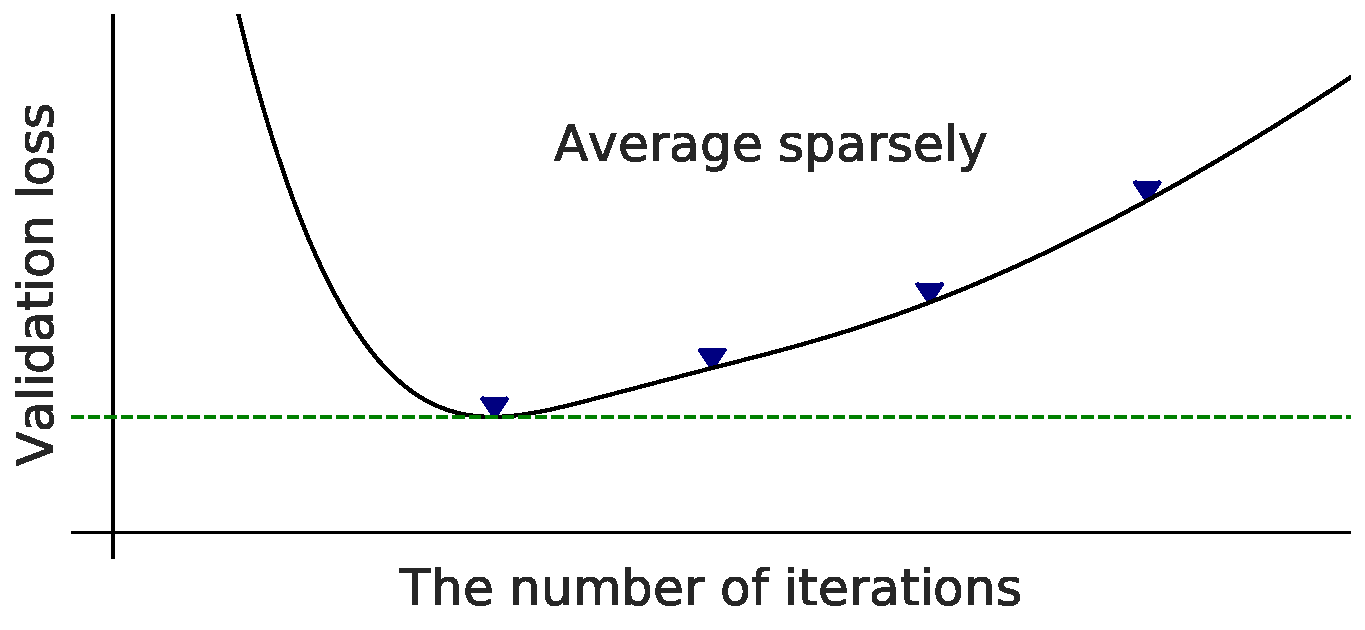
\includegraphics[width=0.4\textwidth]{figures/swad_concept/swa_concept_fig.pdf}%
}
\qquad \quad
\subcaptionbox{\small SWAD\label{fig:swad_overview} (proposed)}{%
  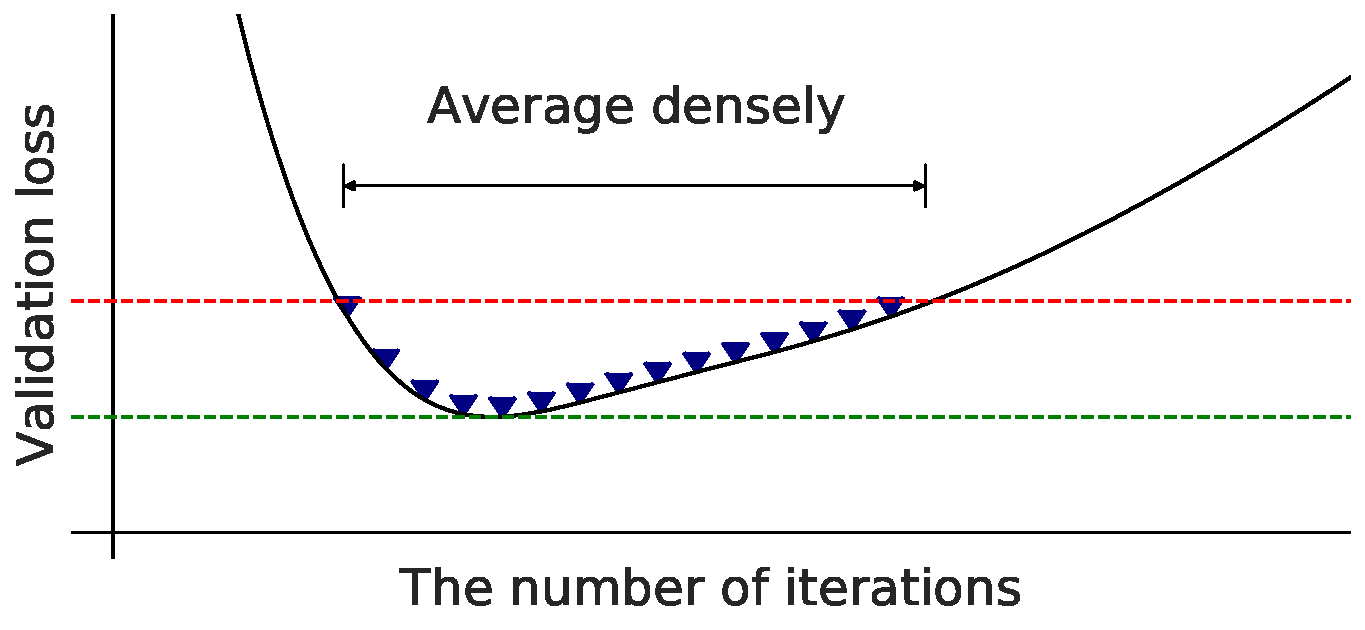
\includegraphics[width=0.4\textwidth]{figures/swad_concept/swad_concept_fig.pdf}%
}
\vspace{-.5em}
\caption{\small {\bf Comparison between SWA and SWAD.} (a) SWA collects stochastic weights for every $K$ epochs from the pre-defined $K_0$ epochs to the final epoch.
% in an interval of certain epoch. 
(b) Our SWAD collects stochastic weights \textbf{\textit{densely}}, \ie, for every iteration, to obtain sufficiently many weights. SWAD collects the weights from the start iteration $t_s$ to the end iteration $t_e$, where $t_s$ and $t_e$ are obtained by monitoring the validation loss (\textbf{\textit{overfit-aware}} scheduling).
% By the proposed dense and overfit-aware gathering strategy, SWAD can collect sufficiently many stochastic weights while avoiding overfitting.
% (b) SWAD computes a threshold from the minimum validation loss, chooses a range from the threshold, and averages all of the weight in the range.}
}
\label{fig:swa_swad_comparison}
\vspace{-1.5em}
\end{figure}